%----------------------------------------------------------------------------------------
%	PACKAGES AND THEMES
%----------------------------------------------------------------------------------------
% handout option removes the pauses
\documentclass[aspectratio=1610,xcolor=dvipsnames]{beamer}
\usetheme{SimplePlus}

\usepackage{tabularx}
\usepackage{hyperref}
\hypersetup{
  colorlinks=true,
  linkcolor=magenta,
  urlcolor=magenta
}
\usepackage{graphicx} % Allows including images
\usepackage{booktabs} % Allows the use of \toprule, \midrule and \bottomrule in tables
\usepackage{listing}  % see style.sty file

%----------------------------------------------------------------------------------------
%	TITLE PAGE
%----------------------------------------------------------------------------------------

\title{Direct Style (for asynchronous programming) in Scala}
\subtitle{The Scala \texttt{gears} library}

\author{Luca Tassinari}

% \institute[NTU] % Your institution as it will appear on the bottom of every slide, may be shorthand to save space
%{
%    Department of Computer Science and Information Engineering \\
%    National Taiwan University % Your institution for the title page
%}
\date{\today} % Date, can be changed to a custom date

%----------------------------------------------------------------------------------------
%	PRESENTATION SLIDES
%----------------------------------------------------------------------------------------

\begin{document}

\begin{frame}
  % Print the title page as the first slide
  \titlepage
\end{frame}

% \begin{frame}{Overview}
%   % Throughout your presentation, if you choose to use \section{} and \subsection{} commands, these will automatically be printed on this slide as an overview of your presentation
%   \tableofcontents
% \end{frame}

%----------------------------------------------------------------------------------------
\section{Context}
%----------------------------------------------------------------------------------------
\begin{frame}{What Direct Style is?}
  \begin{block}{}
    Direct style is a programming style where, in contrast to continuation-passing and monadic styles, the control flow of the program is explicit and the program is written as a sequence of instructions that are executed one after the other, resembling imperative code, while still being in a functional world (with all its advantages!).
  \end{block}
  Advantages:
  \begin{itemize}
      \item It is the most common and natural programming style and every developer is familiar with it;
      \item 
  \end{itemize}
\end{frame}
%
\begin{frame}{Boundary \& Break \cite{scalar-gears}}
  Boundary \& break is a mechanism allowing to prematurely break the computation returning a value to the client: \texttt{boundary} enrich the scope with a \texttt{Label[T]} allowing to \texttt{break} the computation and return a value of type \texttt{T}.
  \lstinputlisting[language=scala]{listings/intro/BoundaryExamples.scala}
  By leveraging boundary \& break it is possible to implement data types to handle errors "directly" with a short exit path. 
\end{frame}
%
\begin{frame}
  \footnotesize
  \texttt{aggregate} returns either the list of HTTP response bodies or the first encountered error.

  \lstinputlisting[language=scala]{listings/intro/DirectAggregate.scala}

  \pause
  Using monadic style:
  \lstinputlisting[language=scala]{listings/intro/MonadicAggregate.scala}

  \pause
  Could be simplified: 
  \lstinputlisting[language=scala]{listings/intro/IdiomaticMonadicAggregate.scala}
\end{frame}
%
\begin{frame}
  \small
  Functions requiring the \texttt{CanFail} type can promptly break the computation upon encountering an error.
  On the calling side, the label is defined using the \texttt{either} boundary.
  
  \lstinputlisting[language=scala]{listings/intro/ShowcasingCanFail.scala}
\end{frame}
%
\begin{frame}[fragile]{Capabilities for modeling effects}
  \begin{block}{}
    Ongoing research project: instead of pushing effects and resources into (monadic) frameworks, upgrade the type system to track them directly in the program $\Rightarrow$ \textbf{CAPabilities for RESources and Effects (CAPRESE)} @ Programming Methods Laboratory EPFL \cite{capabilities}.
  \end{block}
  Idea:
  \begin{itemize}
    \item to have an effect you need the \textbf{capability} enabling it;
    \item a \textit{capability} is just a value passed to the function performing the effect, usually implicitly.
  \end{itemize}
  \texttt{CanFail} is the \textit{capability} enabling the effect of breaking in case of errors:
  \begin{lstlisting}[language=scala, gobble=4]
    def f(using CanFail): Int = ...
  \end{lstlisting}
\end{frame}
%
\begin{frame}<presentation:0>[noframenumbering]
  \fontsize{8}{10}\selectfont
  To model a function with the effect of throwing a \textit{checked} exception
  \footnote{\tiny
    These examples are experimental features of Scala 3 and require to be compiled with \texttt{-experimental} flag or marked as \texttt{@experimental}.
  }:
  \begin{columns}
    \column{0.76\textwidth}
      \lstinputlisting[language=scala]{listings/intro/CanThrow.scala}
    \column{0.2\textwidth}
      \settowidth{\leftmargini}{\usebeamertemplate{itemize item}}
      \addtolength{\leftmargini}{\labelsep}
      \begin{itemize}
        \item This mechanism works only for \textit{checked} exceptions and needs to be enabled with the \texttt{saferExceptions} import.
        \item Unchecked exceptions can still be thrown without the capability.
        \item If the capability is not provided: compilation error!
      \end{itemize}
    \begin{quote}
      \texttt{"The capability to throw exception DivisionByZero is missing."}
    \end{quote}
  \end{columns}
\end{frame}
%
\begin{frame}<presentation:0>[noframenumbering]{Algebraic effects}
  Not just exceptions...
  \begin{block}{}
    Algebraic Effects $\equiv$ exceptions + \texttt{resume} operation \cite{can-throw}
  \end{block}
  The \texttt{resume} operation allows to resume the computation from the point where the effect was raised, after having \textbf{handled} it
  \lstinputlisting[language=scala]{listings/intro/AsyncSupport.scala}
\end{frame}
%
\begin{frame}<presentation:0>[noframenumbering]{Generator effect \cite{scalar-gears}}
  Python-like generator to get all the leafs of a tree:
  \lstinputlisting[language=scala]{listings/intro/TreeGenerator.scala}
\end{frame}
%
\begin{frame}<presentation:0>[noframenumbering]
  \lstinputlisting[language=scala]{listings/intro/Generator.scala}   
\end{frame}
%
\begin{frame}<presentation:0>[noframenumbering]
  \begin{block}{Takeaways}
    \begin{itemize}
      \item Capabilities + delimited continuations enables Algebraic effects
      \begin{itemize}
        \item With algebraic effects, instead of focusing on how to concatenate the effects, we focus on their definition and interpretation (i.e. how to handle them)
      \end{itemize}
      \item Thanks to continuations is possible to design a library for asynchronous computation exploiting \textbf{direct style}, i.e. imperative-like code.
    \end{itemize}
  \end{block}
\end{frame}
%----------------------------------------------------------------------------------------
\section{Scala \texttt{gears}}
%----------------------------------------------------------------------------------------
\begin{frame}{Modeling suspension effect, Scala \texttt{gears} \cite{gears}}
  \begin{block}{}
    Scala \texttt{gears} is a new \textit{experimental} library for asynchronous programming leveraging capabilities to model, with direct style, one of the most important effects: \textbf{\textit{suspension}}.
  \end{block}
  It is designed to be \emph{cross platform}. Currently, it provides suspension support (i.e. the ability to suspend the computation and resume it later) leveraging:
  \begin{itemize}
    \item Virtual Threads on the JVM (requires JRE 21 or later, or JRE 19 with experimental virtual threads enabled);
    \item Delimited continuations on Scala Native.
  \end{itemize}
\end{frame}
%
\begin{frame}
  To introduce the Scala \texttt{scala} gears library, let's consider this very simple example:
  \begin{example}[1]
    We want to program a service allowing storing posts, performing checks on the content and author before the actual storage.
  \end{example}
  Desired behavior:
  \begin{itemize}
    \item the two checks can be spawned and run \textbf{in parallel};
    \item the storage operation should be performed only if both checks succeed;
    \item whenever one of the two fails, \emph{the other gets canceled}!
  \end{itemize}
  \vspace*{0.5cm}
  \footnotesize
  The complete sources of this example are available in the \href{https://github.com/tassiLuca/direct-style-experiments/tree/master/blog-ws-direct}{blog-ws-direct} module.
\end{frame}
%
\begin{frame}[fragile] % needed to insert listing on the fly
  \small
  Both the repository and the service functions are designed to be \textbf{suspendable}:
  \begin{block}{}
    \textbf{The \HL{\texttt{Async}} capability allows a computation to suspend while waiting for the result of an asynchronous source.}
  \end{block}
  \lstinputlisting[language=scala]{listings/example-1/RepositoryService.scala}
  \pause
  \begin{columns}
    \column{0.38\textwidth}
      \HL{\texttt{Async.blocking}} creates an \texttt{Async} context blocking the running thread for suspension (usually placed inside the \texttt{main} or for testing purposes).
    \column{0.6\textwidth}
    \begin{lstlisting}[language=scala,gobble=6]
      @main def launcher(): Unit =
        Async.blocking:
          // here the Async capability is available
    \end{lstlisting}
  \end{columns}
\end{frame}
%
\begin{frame}[fragile]
  \begin{block}{}
    \begin{enumerate}
      \setcounter{enumi}{1}
      \item \texttt{Async.Source} model an asynchronous source of data that can be \textbf{polled} or \textbf{awaited} by suspending the computation, as well as composed using combinator functions.
      \item \texttt{Futures} are the primary (in fact, the only) active elements \textbf{encapsulating a control flow} that, eventually, will deliver a result (either a computed or a failure value that contains an exception)
      \begin{itemize}
        \item To spawn \texttt{Future}s, the \HL{\texttt{Spawn}} capability is needed. It is provided by the \HL{\texttt{Async.group}} function.
        % \begin{lstlisting}[language=scala,gobble=10]
        %   def suspendingFunction(using Async): Int =
        %     Async.group: // needs the Async capability!
        %       // here the Async.Spawn capability is available
        %       Future:
        %         // ...
        % \end{lstlisting}
        %
        % \item \texttt{Tasks} represent delayed \texttt{Futures} (to make them \textit{referential transparent}), essentially wrapping a \texttt{() => Future[T]}.
      \end{itemize}
    \end{enumerate}
  \end{block}
  \pause
  \begin{lstlisting}[language=scala,gobble=4]
    override def create(authorId: AuthorId, title: Title, body: Body)(using Async, CanFail): Post =
      val (post, author) = Async.group: // needs the Async capability!
        // here the Async.Spawn capability is available; hence, we can spawn Futures
        val content = Future(verifyContent(title, body))
        val author = Future(authorBy(authorId))
        ...
  \end{lstlisting}
\end{frame}
%
\begin{frame}
  \begin{columns}
    \column{0.55\textwidth}
      \begin{block}{}
        Every async context has a completion group tracking all computations in a tree structure, enabling \HL{\textbf{structured concurrency}}. 

        Structured concurrency guarantees that \textbf{when a group terminates all its dangling children are canceled}.
      \end{block}
      \begin{itemize}
        \item \texttt{Async.blocking}, \texttt{Async.group} and \texttt{Future} create a new completion group;
        \item to make sure children's computations are not canceled we need to \texttt{await} them.
      \end{itemize}
    \column{0.45\textwidth}
      \begin{figure}
        \centering
        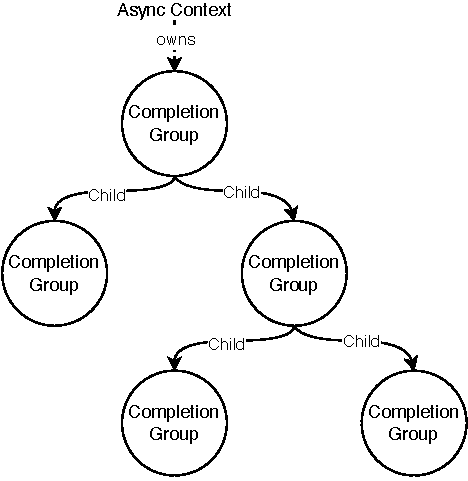
\includegraphics[width=\textwidth]{./images/structured-concurrency.pdf}
      \end{figure}
  \end{columns}
\end{frame}
%
\begin{frame}
  \small
  The complete implementation:
  \lstinputlisting[language=scala]{listings/example-1/PostsServiceImpl.scala}
  \texttt{zip} operator allows combining the results of two \texttt{Future}s in a pair if both succeed, or fail with the first error encountered. Combined with \texttt{Async.group} the failure of one determines the cancellation of the other.
  Note: the only way \texttt{authorBy} and \texttt{verifyContent} can fail, making the \texttt{zip} return immediately the failure (thus cancelling the other check) is by throwing an exception!
\end{frame}
%
\begin{frame}{Sources operators}
  \small
  \begin{table}
    \centering
    \renewcommand{\arraystretch}{1.5}
    \begin{tabular}{ | m{4cm} | m{9cm} | } 
      \hline
      \textbf{Operator} & \textbf{Description} \\
      \hline
      \hline
      \texttt{zip} & Parallel composition of two futures. If both futures succeed, succeed with their values in a pair. Otherwise, fail with the failure that was returned first. \\ 
      \hline
      \texttt{or} & Alternative parallel composition. If either task succeeds, succeed with the success that was returned first. Otherwise, fail with the failure that was returned last (race all futures). \\
      \hline
      \texttt{orWithCancel} & Like \texttt{or} but the slower future is cancelled. \\ 
      \hline
    \end{tabular}
  \end{table}
\end{frame}
%
\begin{frame}
  \begin{columns}[c,onlytextwidth] % The "t" option specifies top vertical alignment
    \column{.35\textwidth}
      \begin{block}{Producer-Consumer pattern}
        The last abstraction: \textbf{Channels}. They represent the primitive communication and coordination means to exchange Future results.
      \end{block}
    \column{.6\textwidth} 
      \begin{figure}
        \centering
        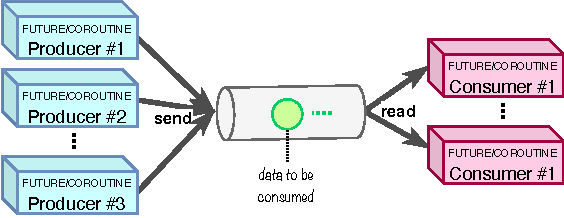
\includegraphics[width=\textwidth]{./images/channels.pdf}
      \end{figure}
  \end{columns}
  \vspace*{1em}
  %\begin{quote}
  %  \centering
  %  \textbf{"Do not communicate by sharing memory; instead, share memory by communicating"} -- Go programming language slogan \cite{effective-go}.
  %\end{quote}
  \small
  \begin{itemize}
      \item Multiple producers and consumers can be "attached" to the same channel;
      \item Consumers compete with each other for sent values;
      \item Once the element is handled, it is immediately removed from the channel;
      \item \texttt{send} and \texttt{read} operations to channels are fair w.r.t. the order of their invocations from multiple process.
  \end{itemize}
\end{frame}
%
\begin{frame}  
  \begin{figure}
    \centering
    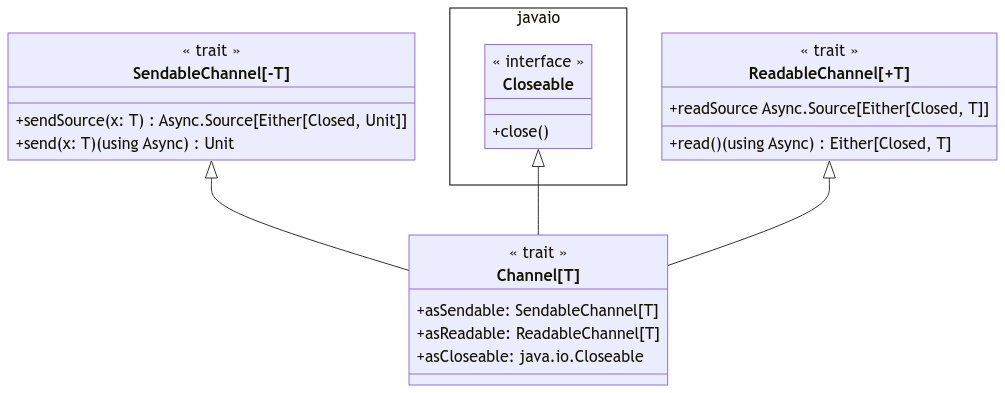
\includegraphics[width=0.7\textwidth]{./images/channels-uml.png}
  \end{figure}
  \begin{itemize}
      \item Synchronous Channels: links a read request to a send within a rendezvous
      \begin{itemize}
          \item \texttt{send} (\texttt{read}) suspend the process until a consumer \texttt{read} (\texttt{send}) the value
      \end{itemize}
      \item Buffered Channels: a version of a channel with an internal buffer of fixed size
      \begin{itemize}
          \item \texttt{send} suspend the process if the channel is full;
          \item \texttt{read} suspend if the channel is empty, waiting for a new value.
      \end{itemize}
      \item Unbounded Channels: a version of a channel with an unbounded buffer
      \begin{itemize}
          \item if the programs run out of memory you can get an out-of-memory exception!
      \end{itemize}
  \end{itemize}
\end{frame}
%
\begin{frame}
  \begin{columns}[c,onlytextwidth]
      \column{.4\textwidth}
        \begin{example}[2]
            We want to realize a little asynchronous library allowing clients to collect the common statistics about repositories (issues, stars, last release) and contributors of a given GitHub organization.
        \end{example}
        \begin{itemize}
            \item Start the computation (interaction with GitHub API is required)
            \item Cancellation of the computation
        \end{itemize}
      %
      \column{.65\textwidth}
        \begin{figure}
            \centering
            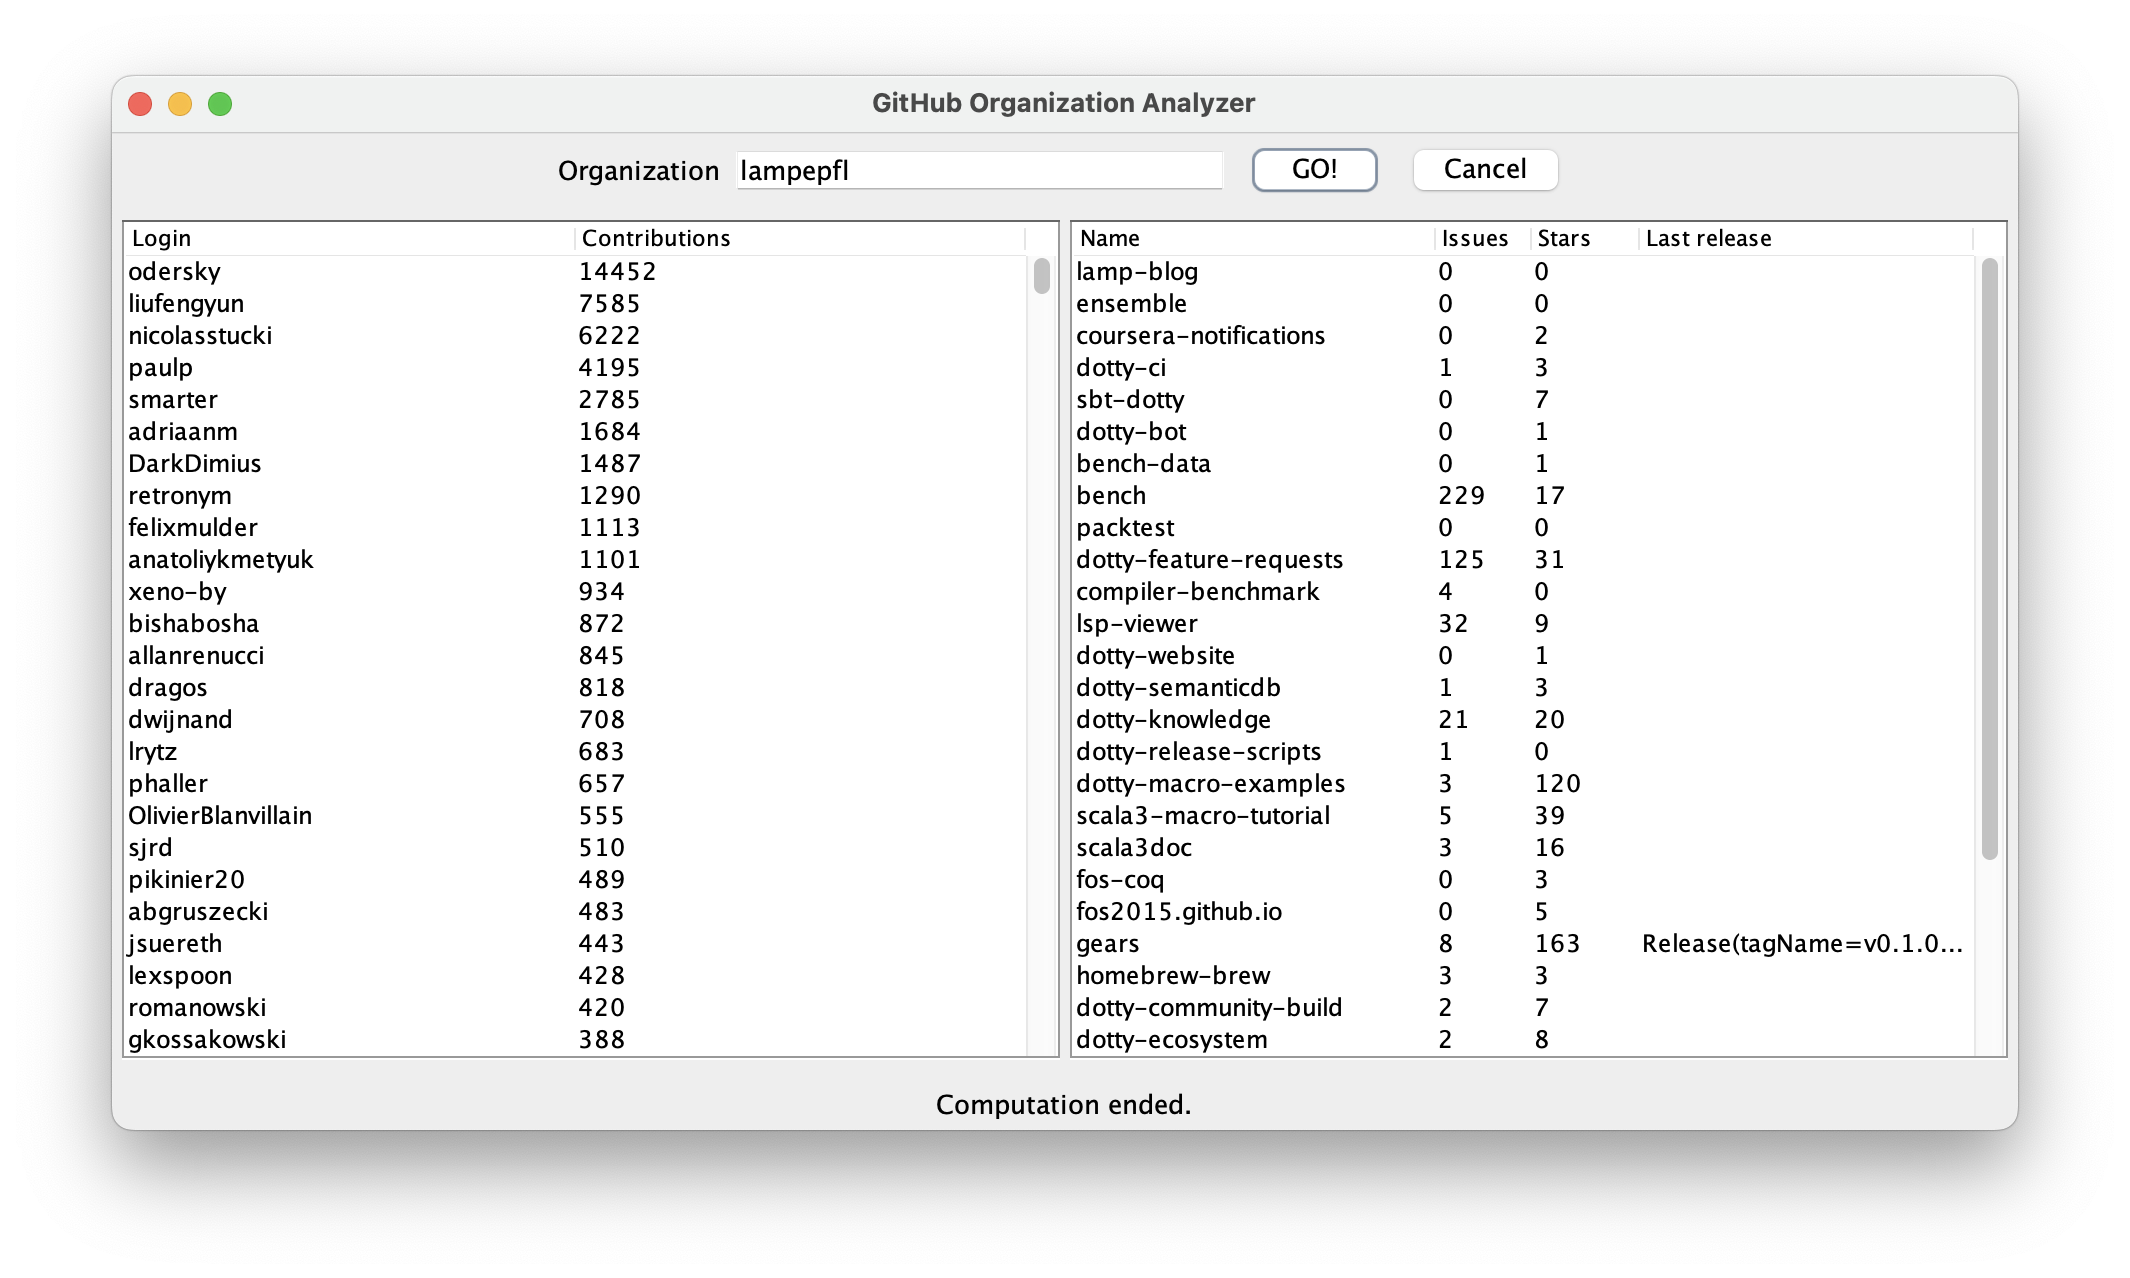
\includegraphics[width=\textwidth]{./images/analyzer-e2e.png}
        \end{figure}
  \end{columns}
  \vspace*{0.5cm}
  \footnotesize
  The complete sources of this example are available in the \href{https://github.com/tassiLuca/direct-style-experiments/tree/master/commons/src}{commons} and \href{https://github.com/tassiLuca/direct-style-experiments/tree/master/analyzer-direct}{analyzer-direct} modules.
\end{frame}
%
\begin{frame}
  The interface of the library provides a suspending method: if the client wants to perform this operation asynchronously, it has to opt in explicitly, using a \texttt{Future}.
  \lstinputlisting[language=scala]{listings/example-2/Analyzer.scala}
  The \texttt{updateResult} is a function allowing the client to react to each incremental result.
\end{frame}
%
\begin{frame}
  \lstinputlisting[language=scala]{listings/example-2/BasicAnalyzer.scala}
  \footnotesize
  \begin{enumerate}
      \item[4)] we get all the repositories of the requested organization
      \item[5)] for each of them, the contributors and the last release are retrieved concurrently, starting a \texttt{Future}
      \item[6)] \texttt{Future} results are gathered within a \texttt{Collector}, which allows a list of \texttt{Future}s to be collected in a channel, arriving as they finish.
      \item[8)] results are read from the channel as they come, calling the \texttt{updateResult} reaction function.
      \item[9)] overall results are returned to the client.
  \end{enumerate}
\end{frame}
%
\begin{frame}[fragile]
  \begin{alertblock}{Problem 1}
    \begin{lstlisting}[language=scala, gobble=6]
      // BLOCKS UNTIL ALL REPOSITORIES HAVE BEEN FETCHED!
      def repositoriesOf(organizationName: String)(using Async, CanFail): Seq[Repository]
    \end{lstlisting}
    \small
    GitHub API implements pagination: if the organization has lots of repositories, the client has to deal with multiple pages of results, but the analysis can start as soon as the first page is retrieved.
  \end{alertblock}
  %
  \pause
  %
  \small$\Rightarrow$ instead of returning a \texttt{Seq[repository]} we return a \texttt{Channel[Repository]}
  %
  \pause
  %
  \begin{alertblock}{Problem 2}
      \small
      Currently, channels are closable, but once closed the consumer cannot finish reading sent values. How to notify no more results are sent?
  \end{alertblock}
  %
  \pause
  %
  \small$\Rightarrow$ \texttt{TerminableChannel}s are introduced in the framework.
  \begin{lstlisting}[language=scala, gobble=4]
    def incrementalRepositoriesOf(
      organizationName: String,
    )(using Async.Spawn): TerminableChannel[Either[String, Repository]]
  \end{lstlisting}
\end{frame}
%
\begin{frame}{TerminableChannel implementation}
  \lstinputlisting[language=scala]{listings/example-2/TerminableChannel.scala}
\end{frame}
%
\begin{frame}
  \lstinputlisting[language=scala]{listings/example-2/TerminableChannelCompanion.scala}
\end{frame}
%
\begin{frame}
  \small
  On top of \texttt{TerminableChannel}s is possible to implement useful methods, like \texttt{foreach} and \texttt{toSeq}:
  \lstinputlisting[language=scala]{listings/example-2/TerminableChannelOps.scala}
\end{frame}
%
\begin{frame}
  \small
  The implementation of the analyzer leveraging \texttt{TerminableChannel}s becomes:
  \lstinputlisting[language=scala]{listings/example-2/IncrementalAnalyzer.scala}
  \footnotesize
  \begin{enumerate}
      \item[5)] iterate over all the repositories sent over the channel as soon as they are retrieved by the service;
      \item[6)] we start the analysis in a separate \texttt{Future}: the analysis is spawned as soon as a repository is fetched by the channel, preventing starting the analysis of the next repository only when the previous one is finished;
      \item[9)] since the analysis are started concurrently the \texttt{updateResult} must be called safely;
      \item[11)] wait for the completion of all the started Futures.
  \end{enumerate}
\end{frame}
%
\begin{frame}
  In this example, \texttt{TerminableChannel}s serve as a workaround for handling an asynchronous computation that generates a stream of values, allowing us to consume them promptly as they become available.
  
  \vspace*{0.5cm}
  $\Rightarrow$ We would like to have a more idiomatic way to handle this kind of computation, possibly in a \textit{referential transparent} way.

  \begin{block}{Kotlin-inspired \texttt{Flow}s}
    They are very similar to cold observable in reactive programming, and they are the perfect fit for functions that need to return a \textbf{stream of asynchronously computed values}. Moreover, thanks to their cold nature, they can be transformed and composed!
  \end{block}
\end{frame}
%
\begin{frame}
  An example of \texttt{Flow} construction: 
  \lstinputlisting[language=scala]{listings/example-2/ShowcasingFlows.scala}
\end{frame}
%
\begin{frame}
  \begin{columns}
    \column{.45\textwidth}
      \lstinputlisting[language=scala]{listings/example-2/ShowcasingFlows2.scala}

      \lstinputlisting[language=scala]{listings/example-2/ShowcasingFlows3.scala}

    \column{.55\textwidth}
      \footnotesize
      [1710596425802] Still not collecting...

      [1710596426807] Starting collecting...

      [1710596427844] Success(Repository(841941,scala/legacy-svn-scala,366,0))

      [1710596427845] Success(Repository(1476202,scala/scala-dist,278,2))

      ...

      [1710596428750] Done!

      \vspace*{0.4cm}

      [1710596865118] Still not collecting...

      [1710596866120] Starting collecting...

      [1710596866383] Failure(java.lang.Exception:\{"message":"Not Found",...\})

      [1710596866383] Done!

      \vspace*{1.2cm}
  \end{columns}
\end{frame}
%
\begin{frame}{Introducing \texttt{Flow}s in \texttt{gears}}
  \lstinputlisting[language=scala]{listings/example-2/Flow.scala}
\end{frame}
%
\begin{frame}
  \lstinputlisting[language=scala]{listings/example-2/FlowCompanionObject.scala}
\end{frame}
%
\begin{frame}
  It is possible to implement useful transformation and combinator functions for manipulating \texttt{Flow}s:
  \lstinputlisting[language=scala]{listings/example-2/FlowOps.scala}
\end{frame}
%
\begin{frame}
  \begin{block}{}
      \begin{itemize}
          \item \texttt{Channel}s are synchronization primitives, used to exchange data between \texttt{Future}s in the same or different process;
          \item \texttt{Channel}s are good for modeling data sources that are \textit{intrinsically hot}, i.e. exist independently of the consumers;
          \item \texttt{Flow}s are perfect for functions that need to return a stream of asynchronously computed values \textit{upon request}. Thanks to their cold nature, they can be transformed and composed.
      \end{itemize}
  \end{block}
\end{frame}
%
\begin{frame}
  \begin{example}[3]
    IoT sensors transmit their measurements to a central hub, which in turn needs to react, in real-time, forwarding to the appropriate controller the data, possibly performing some kind of transformation.
    \begin{figure}
      \centering
      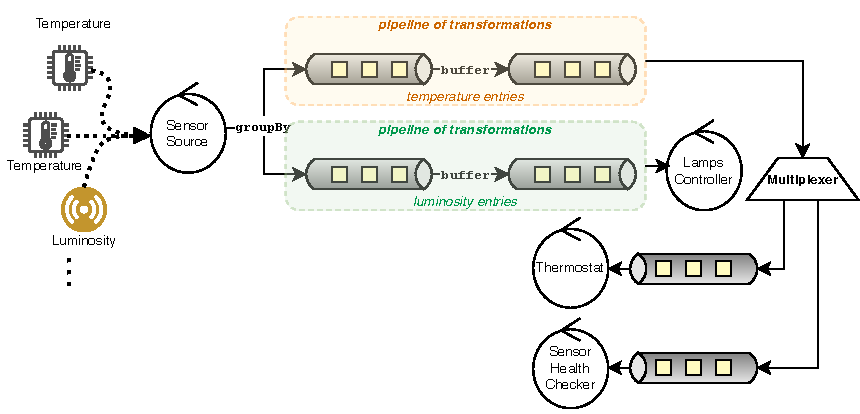
\includegraphics[width=0.8\textwidth]{./images/iot.pdf}
    \end{figure}
  \end{example}
  \footnotesize
  The complete sources of this example are available in the \href{https://github.com/tassiLuca/direct-style-experiments/tree/master/rears/src/main/scala/io/github/tassiLuca/rears}{rears} and \href{https://github.com/tassiLuca/direct-style-experiments/tree/master/smart-hub-direct}{smart-hub} modules.
\end{frame}
%
\begin{frame}
  \small
  \begin{itemize}
    \begin{columns}
      \column{0.5\textwidth}
        \item Tasks provide a way to schedule them using different strategies:
        \begin{itemize}
          \item \texttt{Every}
          \item \texttt{ExponentialBackoff}
          \item \texttt{FibonacciBackoff}
          \item \texttt{RepeatUntilFailure} and \texttt{RepeatUntilSuccess}.
        \end{itemize}
        \item To avoid the work-stealing behavior of channel consumers, a \texttt{ChannelMultiplexer} can be used. It is essentially a container of Readable and Sendable channels, which can be added and removed at runtime.
        \begin{itemize}
          \item Order is guaranteed only per producer;
          \item Typically, the consumer creates a channel and adds it to the multiplexer, then starts reading from it, possibly using a scheduled task.
        \end{itemize}
      \column{0.4\textwidth}
        \begin{figure}
          \centering
          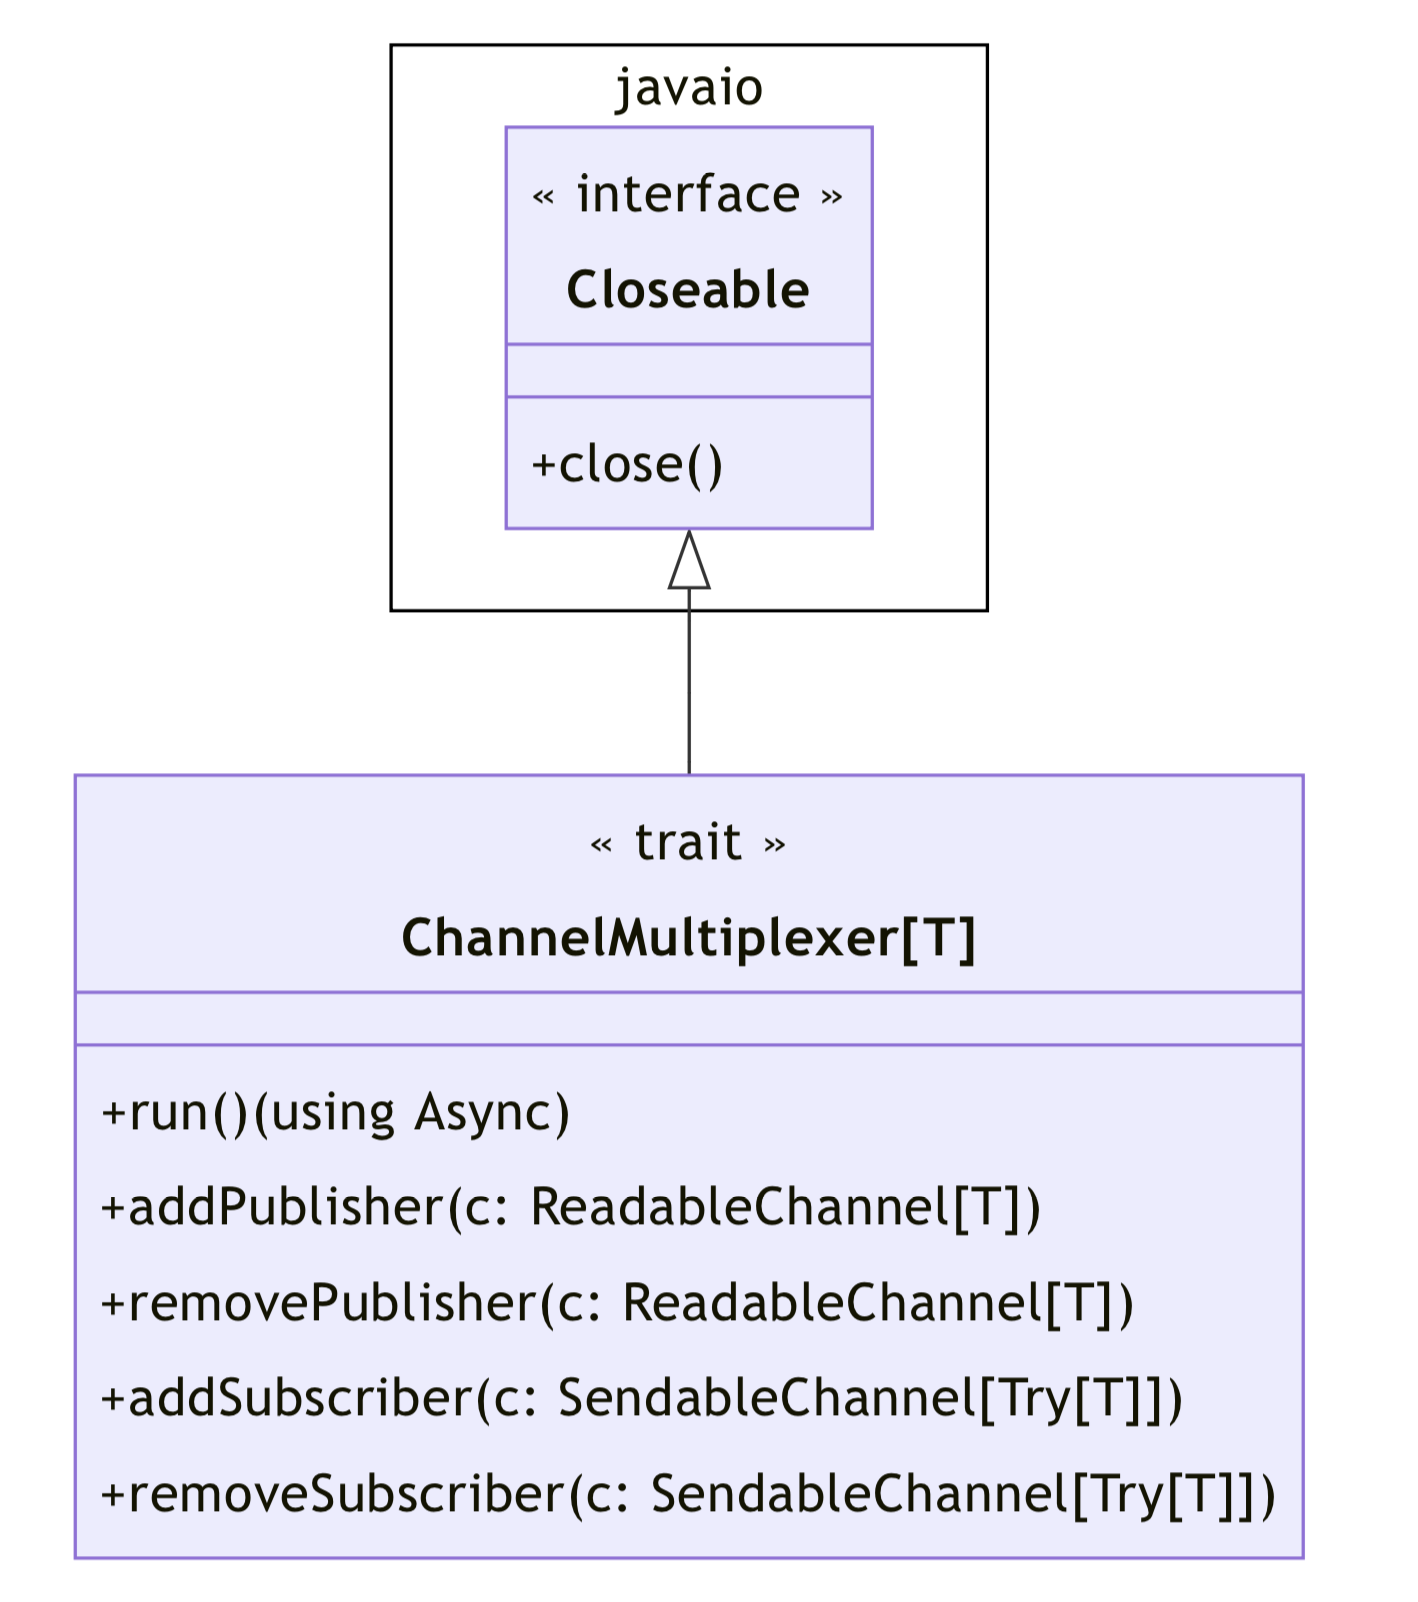
\includegraphics[width=\textwidth]{./images/multiplexer.png}
        \end{figure}
    \end{columns}
  \end{itemize}
  $\Rightarrow$ \texttt{Producer} and \texttt{Consumer} abstractions can be modeled using \texttt{Task} and \texttt{Channel}s.
\end{frame}
%
\begin{frame}
  \lstinputlisting[language=scala]{listings/example-3/ProducerConsumer.scala}
\end{frame}
%
\begin{frame}
  \small
  Now it's possible to model our example in terms of \texttt{Producer}s and \texttt{Consumer}s: the \texttt{SensorSource} is a \texttt{Producer} of \texttt{SensorEvent} publishing sensors data on its \texttt{publishingChannel}:
  \lstinputlisting[language=scala]{listings/example-3/SensorProducer.scala}
\end{frame}
%
\begin{frame}
  \small
  The controllers are \texttt{Consumer} of \texttt{SensorEvent}s. For instance, 
  \texttt{SensorHealthChecker} is a stateful consumer that checks the health of the sensors, sending alerts in case of malfunctioning. Here the state is necessary to determine the health of the sensors, based on the last detection.
  \lstinputlisting[language=scala]{listings/example-3/SensorHealthChecker.scala}
\end{frame}
%
\begin{frame}
  \lstinputlisting[language=scala]{listings/example-3/Controller.scala}
\end{frame}
%
\begin{frame}
  Since Scala \texttt{gears} currently doesn't provide any kind of transformation functions, few of them have been implemented (inspired by Rx):
  \begin{itemize}
      \item \texttt{map}
      \item \texttt{filter}
      \item \texttt{debounce}
      \item \texttt{groupBy}
      \item \texttt{buffer}
      \item \texttt{bufferWithin}
  \end{itemize}
  \footnotesize
  (see \texttt{PipelineTransformations.scala} in the \texttt{rears} module)
\end{frame}
%
\begin{frame}
  \small
  Putting it all together:
  \lstinputlisting[language=scala]{listings/example-3/HubManager.scala}
\end{frame}
%
\begin{frame}
  \small
  To produce a testable version of this example, a simulated source of sensor data has been created, backed to a GUI, through which the user can simulate sensor behavior.
  \begin{figure}
      \centering
      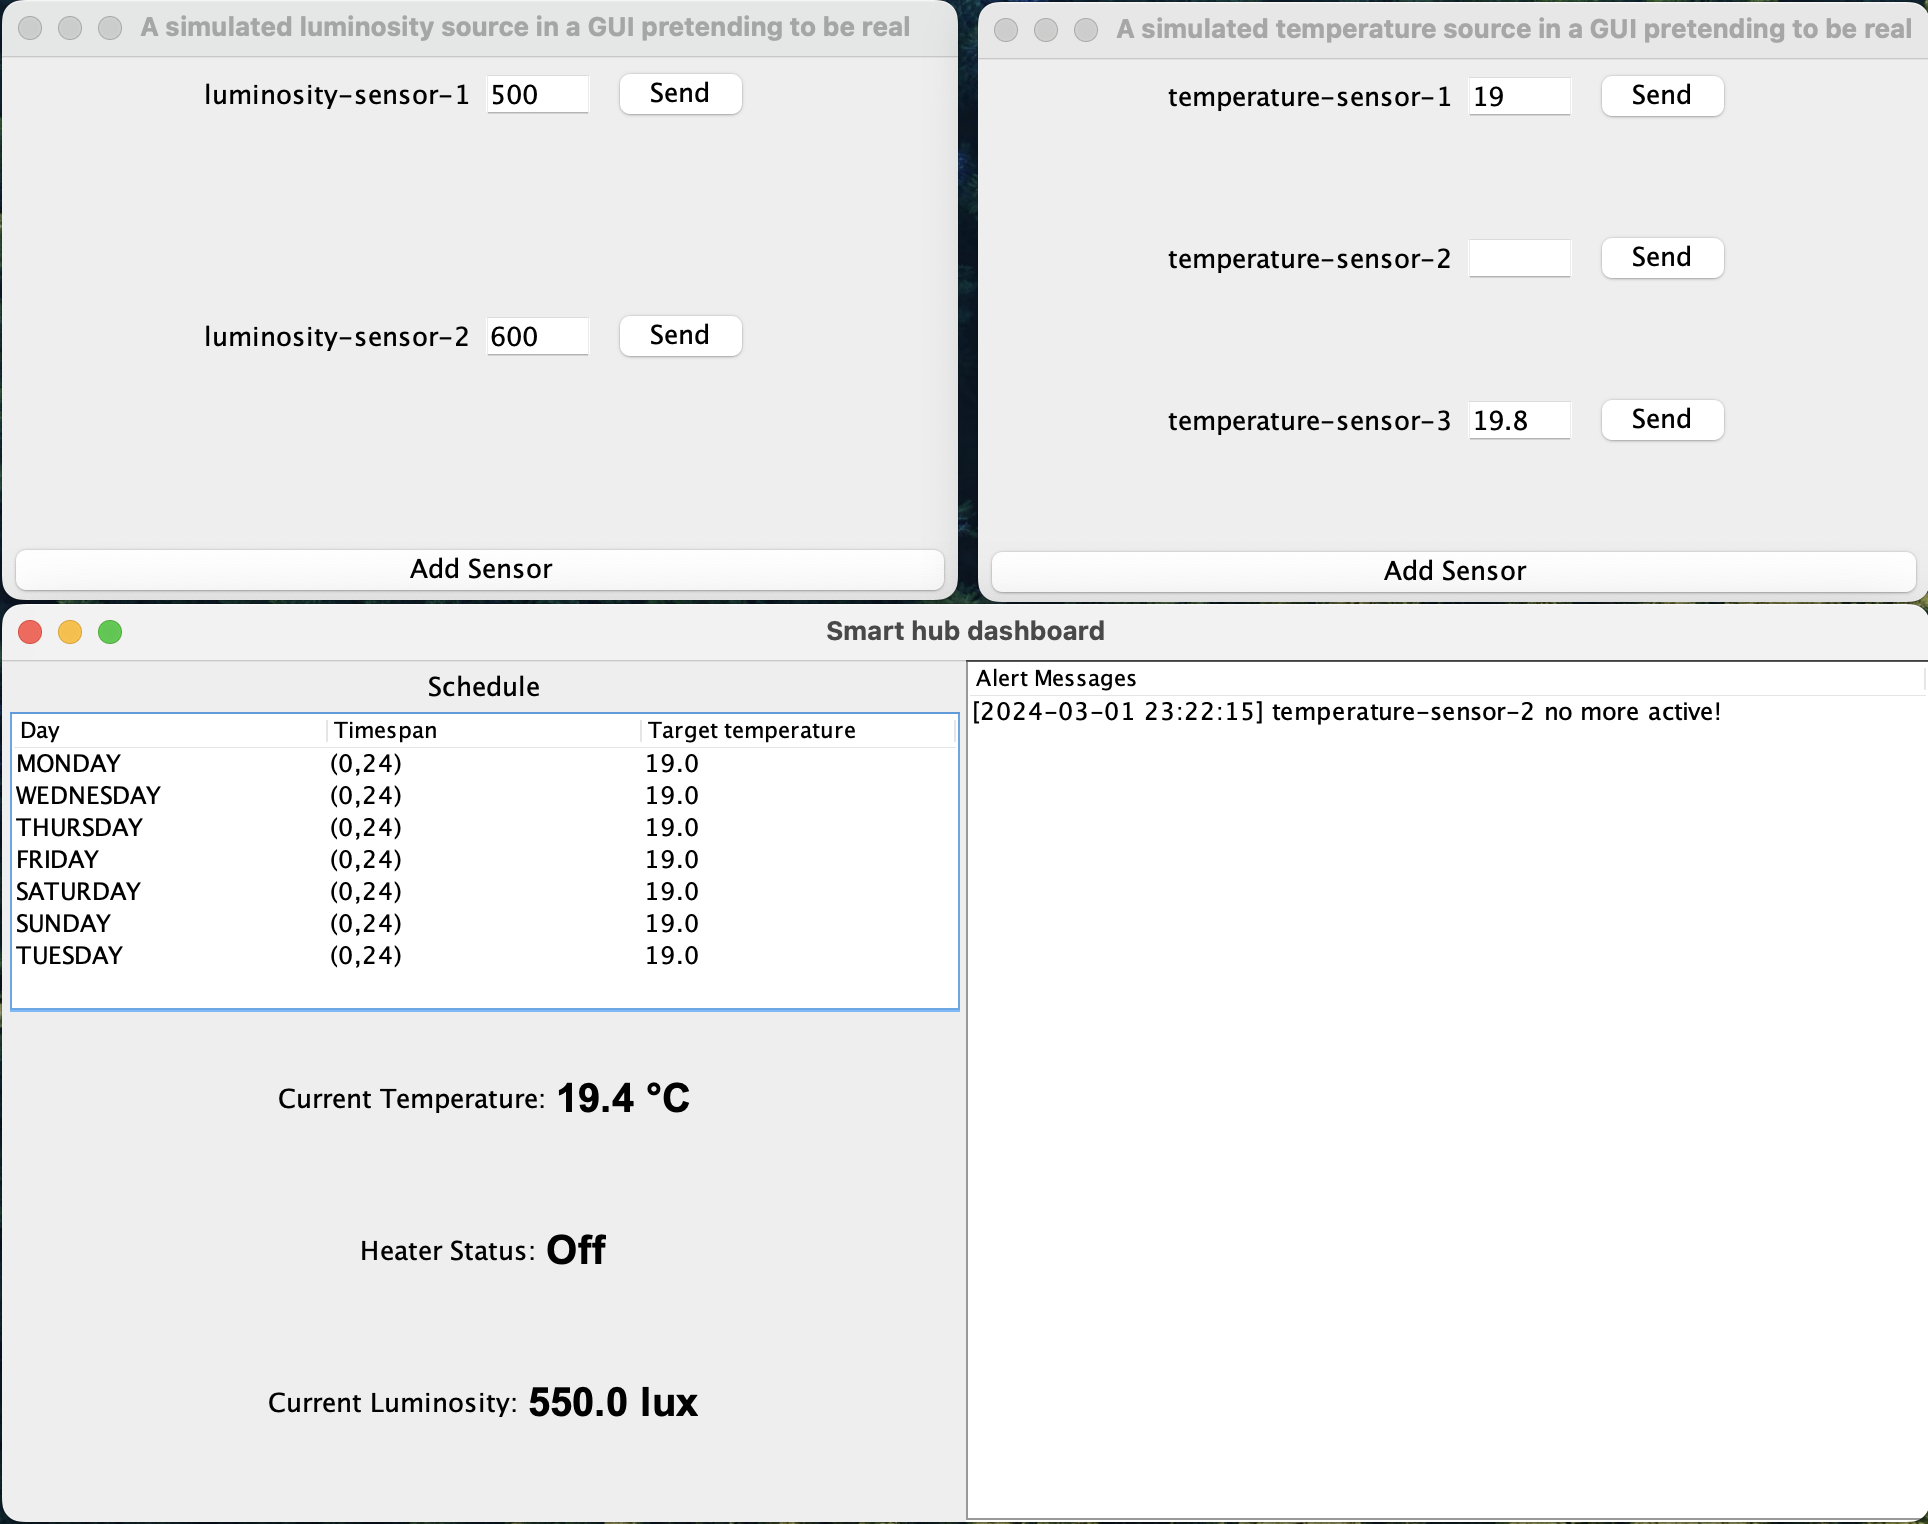
\includegraphics[width=0.6\textwidth]{./images/smart-hub.png}
  \end{figure}
\end{frame}
%
\begin{frame}{Conclusions}
  \begin{itemize}
      \item Direct style frameworks are arising as a natural and intuitive way to handle concurrency, leveraging an imperative-like programming style that is familiar to all developers.
      \item Scala gears, despite being a very young project, provides a good set of abstractions for asynchronous programming, although it cannot yet be considered a mature library ready to be used in a production environment:
      \begin{itemize}
          \item some design choices should be addressed (like closing a channel and the task scheduling)
          \item the library is still missing some important abstractions, like the proposed Flow for handling a cold stream of asynchronously computed values, and operators for functionally transforming channels
          \item  the project has been created for experimenting, thus performances have not been considered a priority so far
      \end{itemize}
  \end{itemize}
\end{frame}
%
\begin{frame}{References}
  % Beamer does not support BibTeX so references must be inserted manually
  \footnotesize{
      \begin{thebibliography}{99}
          \bibitem{capabilities} M. Odersky, A. Boruch-Gruszecki, E. Lee, J. Brachthäuser, O. Lhoták (2022)
          \newblock Scoped Capabilities for Polymorphic Effects
          \newblock \emph{\href{https://doi.org/10.48550/arXiv.2207.03402}{https://doi.org/10.48550/arXiv.2207.03402}}
          %
          %\bibitem{can-throw} CanThrow Capabilities 
          %\newblock Scala 3 nightly documentation
          %\newblock \emph{\href{https://dotty.epfl.ch/docs/reference/experimental/canthrow.html}{https://dotty.epfl.ch/docs/reference/experimental/canthrow.html}}
          %
          \bibitem{scalar-gears} M. Odersky (2023)
          \newblock Direct Style Scala @ Scalar Conference 2023 
          \newblock \emph{\href{https://github.com/lampepfl/gears/blob/main/scalar-slides.pdf}{https://github.com/lampepfl/gears/blob/main/scalar-slides.pdf}}
          %
          \bibitem{gears} Scala \texttt{gears}
          \newblock Programming Methods Laboratory EPFL
          \newblock \emph{\href{https://github.com/lampepfl/gears}{https://github.com/lampepfl/gears}}
          %
          %\bibitem{effective-go}  Effective Go
          %\newblock Share memory by communicating
          %\newblock \emph{\href{https://go.dev/blog/codelab-share}{https://go.dev/blog/codelab-share}}
      \end{thebibliography}
  }
\end{frame}
%----------------------------------------------------------------------------------------
\end{document}
